\documentclass[10pt,aspectratio=169]{beamer}

% Input
\usepackage[utf8]{inputenc}
\usepackage[T1]{fontenc}
\usepackage[letterspace=100]{microtype}
\usepackage{upquote}

% Beamer
\usetheme{metropolis}
\usepackage[sfdefault]{FiraSans}
\usepackage{xcolor}
\definecolor{blue}{HTML}{002957}
\definecolor{red}{HTML}{F1563F}
\setbeamercolor{palette primary}{fg=white,bg=blue}
\setbeamercolor{title separator}{fg=red,bg=blue}
\setbeamercolor{frametitle}{fg=white,bg=blue}
\setbeamercolor{progress bar}{fg=red,bg=blue}
\setbeamercolor{alerted text}{fg=red,bg=blue}
\makeatletter
\setlength{\metropolis@titleseparator@linewidth}{2pt}
\setlength{\metropolis@progressonsectionpage@linewidth}{2pt}
\setlength{\metropolis@progressinheadfoot@linewidth}{2pt}
\makeatother

% Graphics
\usepackage{graphicx}
\usepackage{epstopdf}
\DeclareGraphicsExtensions{.png,.pdf,.eps}

% Various
\usepackage{hyperref}
\usepackage{minted}
\usepackage{fontawesome}

% Title
\title{Beyond Python packaging with Nix}
\subtitle{PyCon PL 2019}
\date{15.9.2019}
\author{Asko Soukka}
\institute{\vspace{0.5cm}
\includegraphics[height=1.5cm]{images/jyu-vaaka-kaksikielinen.eps}}

\newcommand{\setmytemplate}{\usebackgroundtemplate{\begin{picture}(0,0)(-5,250)\footnotesize\href{https://twitter.com/datakurre}{\faTwitter~datakurre} \end{picture}\begin{picture}(0,0)(-355,320)
\includegraphics[width=0.40\paperwidth]{images/nixos-logo-only-hires.png}\end{picture}}}

\begin{document}

\usebackgroundtemplate{\begin{picture}(0,0)(-290,240)
\includegraphics[width=0.30\paperwidth]{images/nixos-logo-only-hires.png}\end{picture}}

\maketitle

\setmytemplate

\section{Hello PyCon PL 2019}

%---------------------------------------------------------------------------------------

\begin{frame}{Asko Soukka}
  \begin{itemize}
    \item Python developer since 2002
    \item Full-time professional since 2008
    \item GSOC mentor since 2013
    \item User of Nix and Docker since 2014
  \end{itemize}
  \begin{itemize}
    \item Plone- and Pyramid-projects
    \item Python microservices
    \item Robot Framework based RPA
  \end{itemize}
\end{frame}

%---------------------------------------------------------------------------------------

\begin{frame}{The Problem}
  \center\Huge
  Python packaging \only<1>{\color{white}{is not enough}}\only<2>{\alert{is not enough}}
\end{frame}

%---------------------------------------------------------------------------------------

\begin{frame}{Robot Framework RPA}
  \textbf{Story}
  \begin{itemize}
    \item Fill a PDF form with provided values
    \item Automate web browser to submit the form
  \end{itemize}
  \textbf{Requirements}
  \begin{itemize}
    \item Robot Framework
    \item PDFtk
    \item Selenium
    \item Firefox
  \end{itemize}
\end{frame}

%---------------------------------------------------------------------------------------

\begin{frame}{RhodeCode SCM}

\includegraphics[width=0.70\paperwidth]{images/rhodecode-tweet.png}
\end{frame}

%---------------------------------------------------------------------------------------

\begin{frame}[fragile]{Standalone Scripts}
  \textbf{Script}
  \begin{minted}{python}
#! /usr/bin/env nix-shell
#! nix-shell -p "python3.withPackages(ps: with ps; [ exifread ])"
#! nix-shell -i python3
from exifread import process_file
print(process_file(open('image.jpg', 'rb')))
  \end{minted}
  \textbf{Executes}
  \begin{minted}{bash}
$ ./script.py
{'Image ImageDescription': (0x010E) ASCII=...
  \end{minted}
  \note{Example: Categorizing photos with exifread}
\end{frame}

%---------------------------------------------------------------------------------------

\setbeamertemplate{background canvas}[default]

%---------------------------------------------------------------------------------------

\begin{frame}[standout]
  \center\Huge
  \alert{Beyond} Python packaging \alert{with Nix}
\end{frame}

%---------------------------------------------------------------------------------------

\setmytemplate

\section{Hello Nix}

\begin{frame}{Nix Ecosystem}
  \textbf{Nix} is a domain-specific, purely functional, lazily-evaluated language for software configuration and deployment.
  \par
  \dotfill
  \begin{itemize}
    \item \textbf{Nix} – purely functional configuration language
    \item \textbf{Nix} – package manager for packages defined in Nix
    \item \textbf{Nixpkgs} – community Nix packages collection
    \item \textbf{NixOS} – Nixpkgs based GNU/Linux distribution
  \end{itemize}
\end{frame}

%---------------------------------------------------------------------------------------

\begin{frame}{Nix History}
  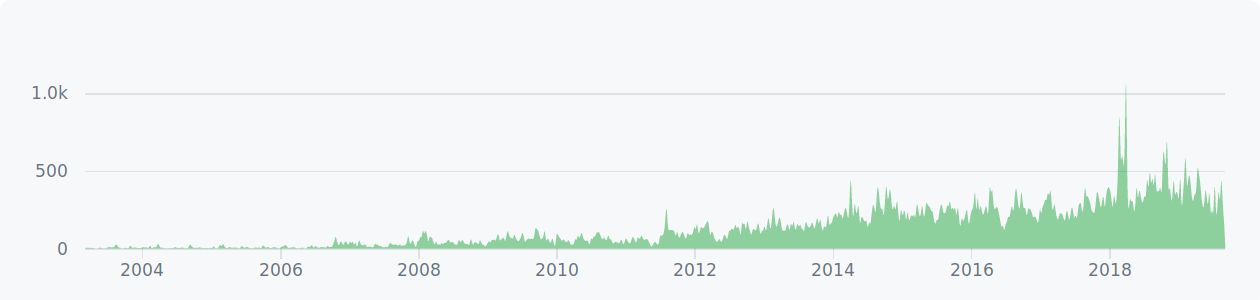
\includegraphics[width=0.9\paperwidth]{images/nixpkgs-graph.png}
  \par
  \begin{itemize}
    \item 2003 Started as a research project by Eelco Dolstra
    \item 2012 Nix 1.0
    \item 2013 NixOS 13.10
  \end{itemize}
\end{frame}

%---------------------------------------------------------------------------------------

\begin{frame}{Nix Today}
  \begin{itemize}
    \item Nix 2.3, NixOS 19.03, \textbf{2,257 all-time contributors}
    \item Nixpkgs has \textbf{over 40 000 packages}
    \item GNU/Linux (i686, \textbf{x86-64}, \textbf{aarch64}), \textbf{macOS}
    \item Supported by NixOS Foundation non-profit
    \item NixCon 2019 25.--27.10. @ Brno, Czech Republic
  \end{itemize}
  \begin{itemize}
    \item \textbf{No official Windows-support yet} \\
    (Cygwin and WLS should work with small effort)
  \end{itemize}
\end{frame}

%---------------------------------------------------------------------------------------

\begin{frame}{Nix Vocabulary}
  Nix \textbf{expressions} are instantiated into \textbf{derivations}, which are realised into build \textbf{outputs}. The collection of build outputs for complete deployment of a software is called \textbf{closure}.
  \par
  \dotfill
  \begin{itemize}
    \item \textbf{Expression} – written Nix-function
    \item \textbf{Derivation} – instantiated expression
    \item \textbf{Output} – build result of a derivation
    \item \textbf{Closure} – the goal of complete deployment
  \end{itemize}
\end{frame}

%---------------------------------------------------------------------------------------

\begin{frame}[fragile]{Nix Expression\hfill1/2}
  \begin{minted}{nix}
{ lib, buildPythonPackage, fetchPypi }:

buildPythonPackage rec {
  pname = "toolz";
  version = "0.10.0";
  src = fetchPypi {
    inherit pname version;
    sha256 = "08fdd5ef7c96480ad11c12d472de21acd...";
  };
  doCheck = false;
}
  \end{minted}
\end{frame}

%---------------------------------------------------------------------------------------

\begin{frame}[fragile]{Nix Expression\hfill2/2}
  \begin{minted}{nix}
with import <nixpkgs> {};
buildEnv {
  name = "env";
  paths = [
    (python37.withPackages (ps: with ps; [
      (callPackage ./toolz.nix {})
      numpy
    ]))
    graphviz
  ];
}
  \end{minted}
\end{frame}

%---------------------------------------------------------------------------------------

\begin{frame}{Python Closure\hfill1/2}
\vspace{0.71cm}
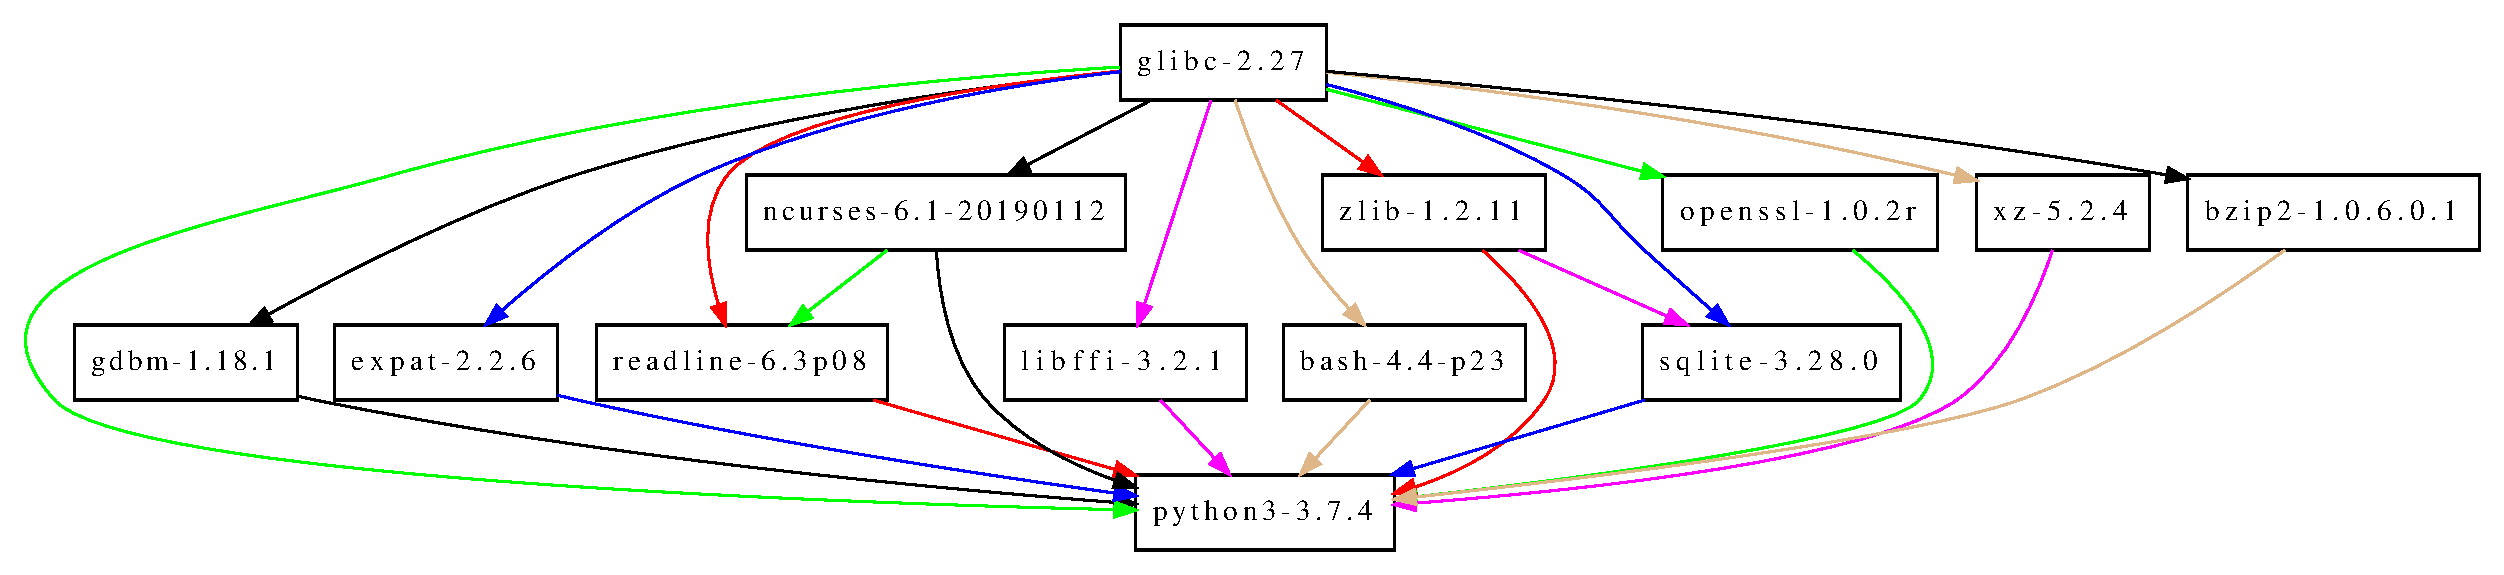
\includegraphics[trim=300 0 0 0,height=0.72\paperheight]{images/python-closure.eps}
\end{frame}

%---------------------------------------------------------------------------------------

\begin{frame}[fragile]{Python Closure\hfill2/2}
  \begin{minted}{bash}
/nix/store/96p426c8n8k16j-python3-3.7.4
+---/nix/store/681354n3k44r8z90m35hm8945vsp95h1-glibc-2.27
|   +---/nix/store/681354n3k44r8z90m35hm8945vsp95h1-glibc-2.27 [...]
+---/nix/store/26ani5lvmf4yanr8m7jc1z3irdk16yqg-gdbm-1.18.1
|   +---/nix/store/681354n3k44r8z90m35hm8945vsp95h1-glibc-2.27 [...]
|   +---/nix/store/26ani5lvmf4yanr8m7jc1z3irdk16yqg-gdbm-1.18.1 [...]
+---/nix/store/...-ncurses-6.1-20190112
|   +---/nix/store/...-glibc-2.27 [...]
|   +---/nix/store/...-ncurses-6.1-20190112 [...]
+---/nix/store/...-readline-6.3p08
|   +---/nix/store/...-glibc-2.27 [...]
|   +---/nix/store/...-ncurses-6.1-20190112 [...]
  \end{minted}
\end{frame}

%---------------------------------------------------------------------------------------

\begin{frame}{Not Unlike Conda}
\vspace{0.2cm}

\includegraphics[width=0.6\paperwidth]{images/nix-conda-tweet.png}
\end{frame}

%---------------------------------------------------------------------------------------

\begin{frame}{Much Batteries}
  Nix expressions \textbf{compose} together unlike anything to allow goodies like:
  \begin{itemize}
    \item TeX Live environment tools
    \item Container image tools
    \item Cross-compilation tools
    \item NixOS image building tools
    \item KVM based system test tools
    \item \ldots
  \end{itemize}
\end{frame}

%---------------------------------------------------------------------------------------

\setbeamertemplate{background canvas}[default]

% YOLO, Rasbperry PI

%---------------------------------------------------------------------------------------

\begin{frame}[standout]
\vfill

\includegraphics[height=0.50\paperheight]{images/nixos-logo-white-hires.png}
\end{frame}

%---------------------------------------------------------------------------------------

\setmytemplate

%---------------------------------------------------------------------------------------

\section{Installing Nix}

%---------------------------------------------------------------------------------------

\begin{frame}[fragile]{Single-User Installation}
  \textbf{Install}

  \begin{minted}{bash}
  $ sudo mkdir /nix
  $ sudo chown username /nix
  $ sh <(curl https://nixos.org/nix/install) --no-daemon
  \end{minted}

  \textbf{Uninstall}

  \begin{minted}{bash}
  $ rm -rf /nix
  \end{minted}
\end{frame}

%---------------------------------------------------------------------------------------

\begin{frame}[fragile]{Installation Errors}

  \textbf{When this happens}

  \begin{minted}{bash}
  error: cloning builder process: Invalid argument
  error: unable to start build process
  babblebabblebabble...
  \end{minted}

  \textbf{Disable sandboxed builds}

  \begin{minted}{bash}
  $ mkdir -p ~/.config/nix
  $ echo "sandbox = false" > ~/.config/nix/nix.conf
  \end{minted}

  \textbf{Or ask help}

  \begin{itemize}
    \item \href{https://discourse.nixos.org/}{https://discourse.nixos.org/}
  \end{itemize}

\end{frame}

%---------------------------------------------------------------------------------------

\section{nix-env}

%---------------------------------------------------------------------------------------

\begin{frame}[fragile]{Nix User Environment\hfill1/4}

  \textbf{Search available packages}
  \begin{minted}{bash}
  $ nix search python37
  * nixpkgs.python37 (python3)
    A high-level dynamically-typed programming language
  \end{minted}

  \textbf{Install found packages}
  \begin{minted}{bash}
  $ nix-env -iA nixpkgs.python37
  installing 'python3-3.7.4'
  \end{minted}

\end{frame}

%---------------------------------------------------------------------------------------

\begin{frame}[fragile]{Nix User Environment\hfill2/4}

  \textbf{List installed packages}
  \begin{minted}{bash}
  $ nix-env -q
  python3-3.7.4
  \end{minted}

  \textbf{Uninstall packages}
  \begin{minted}{bash}
  $ nix-env -e python3
  uninstalling 'python3-3.7.4'
  \end{minted}

\end{frame}

%---------------------------------------------------------------------------------------

\begin{frame}[fragile]{Nix User Environment\hfill3/4}

  \textbf{Update configured channels}
  \begin{minted}{bash}
  $ nix-channel --update
  unpacking channels...
  \end{minted}

  \textbf{Upgrade installed packages}
  \begin{minted}{bash}
  $ nix-env -u
  upgrading 'python3' to 'python3-3.7.4'
  \end{minted}

\end{frame}

%---------------------------------------------------------------------------------------

\begin{frame}[fragile]{Nix User Environment\hfill4/4}

  \textbf{Install Python with packages}
  \begin{minted}{bash}
  $ nix-env -f "<nixpkgs>" -i -E \
    "f: (f {}).python37.withPackages(ps: with ps; [ numpy ])"
  \end{minted}

  \textbf{Rollback to previous state}
  \begin{minted}{bash}
  $ nix-env --rollback
  switching from generation 3 to 2
  \end{minted}

\end{frame}

%---------------------------------------------------------------------------------------

\section{nix-shell}

%---------------------------------------------------------------------------------------

\begin{frame}[fragile]{Ad-hoc Nix-shell\hfill1/3}

  \textbf{Activate nix-shell}
  \begin{minted}{bash}
  $ nix-shell -p python37
  [nix-shell:~]$ which python
  /nix/store/...--python3-3.7.4/bin/python
  \end{minted}

  \textbf{Use without activation}
  \begin{minted}{bash}
  $ nix-shell -p python37 --run "python --version"
  Python 3.7.4
  \end{minted}

\end{frame}

%---------------------------------------------------------------------------------------

\begin{frame}[fragile]{Ad-hoc Nix-shell\hfill2/3}

  \textbf{Activate pure nix-shell}
  \begin{minted}{bash}
  $ nix-shell --pure -p python37
  [nix-shell:~]$ which python
  /nix/store/...--python3-3.7.4/bin/python
  \end{minted}

  \textbf{Use purely without activation}
  \begin{minted}{bash}
  $ nix-shell --pure -p python37 --run "python --version"
  Python 3.7.4
  \end{minted}

\end{frame}

%---------------------------------------------------------------------------------------

\begin{frame}[fragile]{Ad-hoc Nix-shell\hfill3/3}

  \textbf{Activate Nix-shell with Python environment}
  \begin{minted}{bash}
  $ nix-shell -p "python37.withPackages(ps: [ ps.numpy ])"
  [nix-shell:~]$ python -c "import numpy; print(numpy)"
  <module 'numpy' from '/nix/store/...-python3-3.7.4-env/...'>
  \end{minted}

  \textbf{Cleanup downloads and builds}
  \begin{minted}{bash}
  $ nix-collect-garbage
  \end{minted}

\end{frame}

%---------------------------------------------------------------------------------------

\begin{frame}[fragile]{Nix-shell as Script Interpreter}
  \textbf{Nix-shell} can be used as a script interpreter to execute a script with the requirements (\texttt{-p}) and interpreter (\texttt{-i}) defined in the script itself.
  \begin{minted}{python}
#! /usr/bin/env nix-shell
#! nix-shell -p "python3.withPackages(ps: with ps; [ scikitlearn ])"
#! nix-shell -i python3
from sklearn import datasets
iris = datasets.load_iris()
digits = datasets.load_digits()
  \end{minted}
\end{frame}

%---------------------------------------------------------------------------------------

\begin{frame}[fragile]{Managed Nix-shell\hfill1/3}
  \textbf{Nix-shell} defaults to build the shell from \texttt{./shell.nix} .
  \begin{minted}{nix}
with import <nixpkgs> {};
mkShell {
  buildInputs = [
    (python37.withPackages (ps: with ps; [
      scikitlearn
    ]))
    gnumake
  ];
}
  \end{minted}
\end{frame}

%---------------------------------------------------------------------------------------

\begin{frame}[fragile]{Managed Nix-shell\hfill2/3}

  \textbf{Activate nix-shell}
  \begin{minted}{bash}
  $ nix-shell
  \end{minted}

  \textbf{Use without activation}
  \begin{minted}{bash}
  $ nix-shell --run "make check"
  \end{minted}

  \textbf{Use at Travis-CI}
  \begin{minted}{yaml}
language: nix
script: nix-shell --run "make check"
  \end{minted}

\end{frame}

%---------------------------------------------------------------------------------------

\begin{frame}[fragile]{Managed Nix-shell\hfill3/3}
  Ensure \textbf{reproducibility by locking} to exact Nixpkgs revision.
  \begin{minted}{nix}
with import (builtins.fetchTarball {
  url = "https://github.com/NixOS/nixpkgs-channels/archive/....tar.gz";
  sha256 = "0h3s9sn0fzq31hgig5yhcw1pnr7kc7cchixn5b85rgvm70nrwhi6";
}) {};
mkShell {
  ...
}
  \end{minted}
  Hash can be precalculated with \texttt{nix-prefetch-url -{}-unpack} .
\end{frame}

%---------------------------------------------------------------------------------------

\section{nix-build}

%---------------------------------------------------------------------------------------

\begin{frame}[fragile]{Nix-build\hfill1/2}
  Assuming a project environment defined in \texttt{./env.nix}
  \begin{minted}{nix}
with import <nixpkgs> {};
buildEnv {
  name = "env";
  paths = [(python37.withPackages (ps: with ps; [ scikitlearn ]))];
}
  \end{minted}
  \textbf{nix-build} can realise the environment into an \textbf{output link}.
  \begin{minted}{bash}
  $ nix-build env.nix -o env
  \end{minted}
\end{frame}

%---------------------------------------------------------------------------------------

\begin{frame}[fragile]{Nix-build\hfill2/2}
  Nix-build output link (e.g. \texttt{./env}) doubles as a \textbf{garbage collector lock}.
  \begin{minted}{bash}
  $ stat -c '%N' ./env
  'env' -> '/nix/store/f1yia0prn3a8n16da0lwa4hfdgaw055z-env'
  \end{minted}
  \begin{minted}{bash}
  $ stat -c '%N' /nix/var/nix/gcroots/auto/bkd0...
  '/nix/var/nix/gcroots/auto/...' -> '/home/.../env'
  \end{minted}
  Remove the output link to allow \texttt{nix-collect-garbage} \\
  to collect the build output (and free some disk space).
\end{frame}

%---------------------------------------------------------------------------------------

\section{Nix dockerTools}

%---------------------------------------------------------------------------------------

\begin{frame}[fragile]{Nix dockerTools\hfill1/3}
  Nixpkgs' \textbf{dockerTools} provide expressions for creating Docker images.
  \begin{minted}{nix}
with import <nixpkgs> {};
dockerTools.buildLayeredImage {
  name = "acme";
  tag = "latest";
  contents = [
    (import ./env.nix)
    busybox
  ];
}
  \end{minted}
\end{frame}

%---------------------------------------------------------------------------------------

\begin{frame}[fragile]{Nix dockerTools\hfill2/3}
  Image is built with \textbf{nix-build} and loaded to use with \textbf{Docker}.
  \par
  \vspace{0.5cm}
  \begin{minted}{bash}
  $ docker load < $(nix-build docker.nix)
  Loaded image: acme:latest
  \end{minted}
  \par
  \vspace{0.5cm}
  Calling nix-build results in a new build only if any of the dependencies\\have changed. Everything gets cached in \texttt{/nix/store} as usual with Nix.
\end{frame}

%---------------------------------------------------------------------------------------

\begin{frame}[fragile]{Nix dockerTools\hfill3/3}
  \begin{minted}{nix}
with import <nixpkgs> {};
dockerTools.buildImage {
  ...
  runAsRoot = ''
    #!${pkgs.stdenv.shell}
    ${pkgs.dockerTools.shadowSetup}
    groupadd --system --gid 65543 nobody
    useradd --system --uid 65543 --gid 65543 -d / -s /sbin/nologin nobody
  '';
  config = { User = "nobody"; };
  keepContentsDirlinks = true;
}
  \end{minted}
\end{frame}

%---------------------------------------------------------------------------------------

\section{Python Packaging in Nix}

%---------------------------------------------------------------------------------------

\begin{frame}[fragile]{Packaging Python Application}
  \begin{minted}{nix}
with import <nixpkgs> {};

python3Packages.buildPythonApplication {
  pname = "hello-world";
  version = "1.0.0";
  src = lib.cleanSource ./.;
# nativeBuildInputs = [];
# checkInputs = [];
# buildInputs = [];
# propagatedBuildInputs = [];
}
  \end{minted}
\end{frame}

%---------------------------------------------------------------------------------------

\begin{frame}[fragile]{Packaging with Dependencies}
  \begin{minted}{nix}
with import <nixpkgs> {};

let self = rec {
  my_lib = python3Packges.buildPythonPackage { ... };
};
in python3Packages.buildPythonApplication {
  ...
  propagatedBuildInputs = with self; [
    my_lib
  ];
}
  \end{minted}
\end{frame}

%---------------------------------------------------------------------------------------

\begin{frame}[fragile]{Generating Python Packages}
  \textbf{pypi2nix}
  \begin{itemize}
    \item \href{https://github.com/nix-community/pypi2nix}{github.com/nix-community/pypi2nix}
    \item No re-use of Python packages in Nixpkgs
  \end{itemize}
  \textbf{setup.nix}
  \begin{itemize}
    \item \href{https://github.com/nix-community/setup.nix}{github.com/nix-community/setup.nix}
    \item Overlays on top of Python packages in Nixpkgs
  \end{itemize}
\end{frame}

%---------------------------------------------------------------------------------------

\begin{frame}[fragile]{First image of a black hole: Python DIY }
\textbf{Nix-packaging and Travis-CI example}\\
\href{https://github.com/datakurre/EHTM87/}{github.com/datakurre/EHTM87}
\par

\includegraphics[width=0.20\paperwidth]{images/M87.png}
\par
by following the instructions given by Maciej Wielgus.
\end{frame}

%---------------------------------------------------------------------------------------

\begin{frame}{Nix Resources}
  \textbf{Official resources}
  \begin{itemize}
    \item \href{https://nixos.org/}{https://nixos.org/}
    \item \href{https://nixos.org/nix/manual/}{https://nixos.org/nix/manual/}
    \item \href{https://nixos.org/nixpkgs/manual/}{https://nixos.org/nixpkgs/manual/}
  \end{itemize}
  \textbf{Community resources}
  \begin{itemize}
    \item \href{https://github.com/nix-community/awesome-nix/}{https://github.com/nix-community/awesome-nix/}
    \item \href{https://discourse.nixos.org/}{https://discourse.nixos.org/}
    \item \#nixos @ Freenode
  \end{itemize}
\end{frame}

%---------------------------------------------------------------------------------------

\setbeamertemplate{background canvas}[default]

\begin{frame}[standout]
\vfill

\includegraphics[height=0.50\paperheight]{images/pyconplhearts.png}
\par
\href{https://datakurre.github.io/pyconpl19/}{datakurre.github.io/pyconpl19}
\end{frame}

%---------------------------------------------------------------------------------------

\end{document}
